\chapter{MOS Overview}

\section{Current with modulation effect}

\begin{equation}
I_{DS}=\frac{1}{2}\mu C'_{ox}\frac{W}{L}(V_{GS}-V_t)^2 (1+\frac{V_D-V_S}{V_A})
\end{equation}

\section{Weak inversion regime}

\centering
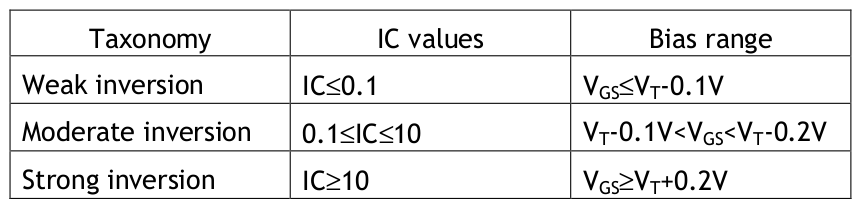
\includegraphics[width=0.55\textwidth]{Schermata.png}\\
\raggedright

\subsection{Inversion Coefficient IC}
\begin{equation}
IC=\frac{I}{2n\mu C'_{ox}V_{th}^2 W/L}
\end{equation}
With n=1.5 subthreshold coefficient.\\

\subsection{Transconductance}
\begin{equation}
g_m=\frac{I}{nV_{th}}\frac{2}{1+\sqrt{1+4IC}}
\end{equation}

\section{Cut-off frequency}
\begin{equation}
f_t=\frac{g_m}{2\pi(C_{gs}+C_{gd})}
\end{equation}

\section{Saturation conditions}

\centering
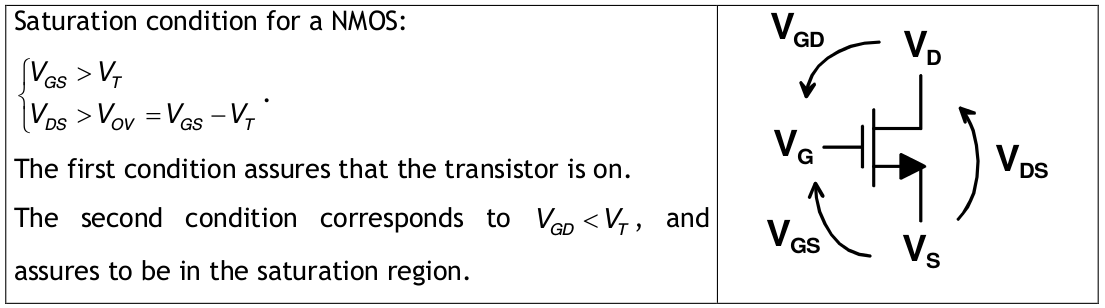
\includegraphics[width=0.7\textwidth]{nmossat.png}\\
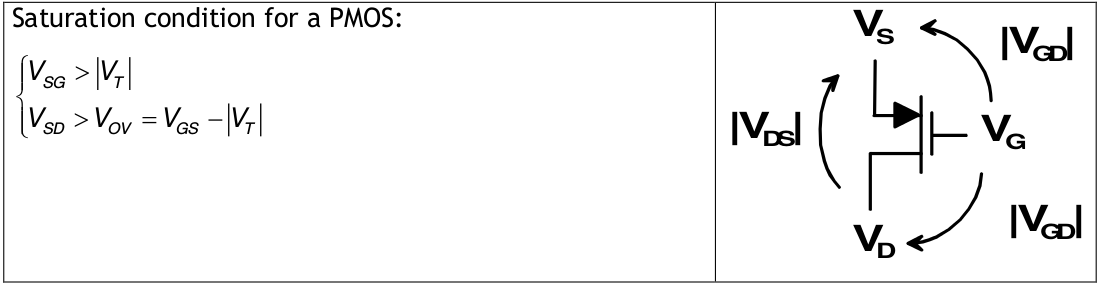
\includegraphics[width=0.7\textwidth]{pmossat.png}\\
\raggedright


\section{Input and output resistance in MOS circuits}

\centering
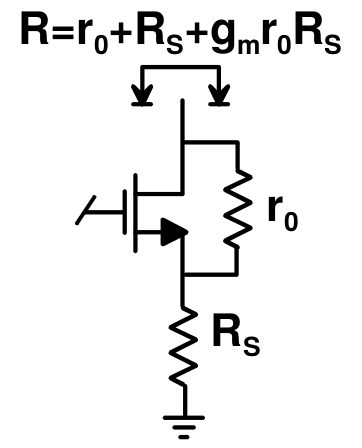
\includegraphics[width=0.25\textwidth]{dres.png}
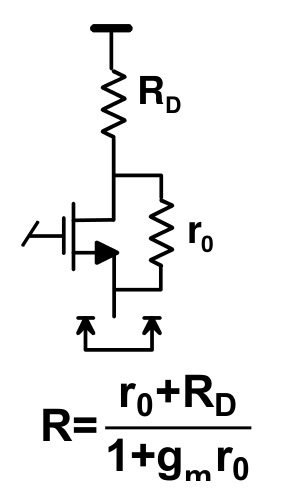
\includegraphics[width=0.2\textwidth]{sres.png}\\
\raggedright

\section{Pelgrom costants}
\subsection{For resistors}
\begin{equation}
\frac{\Delta R}{R}=\frac{K_{\Delta R / R}}{\sqrt{WL}}
\end{equation}
\subsection{For transistors}
{\bf Threshold voltage}\\
\begin{equation}
\sigma(\Delta V_t)=\frac{K_{\Delta V_t / V_t}}{\sqrt{WL}}
\end{equation}
{\bf Parameter k}\\
\begin{equation}
\sigma(\frac{\Delta k}{k})=\frac{K_{\Delta V_t / V_t}}{\sqrt{WL}}
\end{equation}
